\chapter{Evaluation}\markright{Chapter 5: Evaluation}\label{sec:evaluation} 
In order to demonstrate the effectiveness of \our scheme, \We evaluate Accuracy, True Positive Rate (TPR), and False Positive Rate (FPR) among the several schemes shown in \tablename~\ref{tab:schemes} with real datasets. 
As shown in \tablename~\ref{tab:schemes}, the permission besed scheme utilizes only binary features regarding the presence of dangerous permissions.
If an app has a dangerous permission, the feature regarding the permission is 1.
Otherwise the feature is zero.  
Meanwhile, SSL certificate based scheme uses SSL server certificate based features without permission based weight.
Accuracy, TPR, FPR are calculated as:
\begin{equation}
  \mathrm{Accuracy} = \frac{\mathrm{TP}+\mathrm{TN}}{\mathrm{TP} + \mathrm{TN} + \mathrm{FP} + \mathrm{FN}}, 
\end{equation}
\begin{equation}
  \mathrm{TPR} = \frac{\mathrm{TP}}{\mathrm{TP + FN}},
\end{equation}
\begin{equation}
  \mathrm{FPR} = \frac{\mathrm{FP}}{\mathrm{FP + TN}},
\end{equation}
where TP, TN, FP, and FN denote the number of True Positive (malwares are regarded as malwares), True Negative (benign apps are regarded as benign ones), False Positive (benign apps are regarded as malwares), and False Negative (malwares are regarded as benign apps), respectively.  

\begin{table}[p]
  \begin{center}
    \vspace{-8pt} 
    \caption{The schemes used for the evaluation}
    \label{tab:schemes} 
    % \vspace{-8pt} 
    % \hspace{-10pt} 
    \begin{tabular}{|c|c|c|c|c|} \hline
      \multirow{3}{*}{\hfill Schemes \hfill} & \multicolumn{4}{c|}{The name of parameters used in our evaluation}  \\ \cline{2-5} 
                                             & SSL server  & weight & Previous & Dangerous \\ 
                                             & certificate & value & features & permissions \\ \hline \hline
      % Prop.1 & $\checkmark$&$\checkmark$ && \\ \cline{1-5} 
      \Our scheme & $\checkmark$&$\checkmark$ && \\ \cline{1-5} 
      Previous scheme & & & \checkmark &\\ \cline{1-5} 
      % Prop.2 & $\checkmark$ & & & \\ \cline{1-5} 
      SSL certificate  & \multirow{2}{*}{$\checkmark$} & & & \\  
      besed scheme & & & &  \\ \cline{1-5} 
      % Prop.3 & $\checkmark$ & $\checkmark$ & $\checkmark$ & \\ \cline{1-5} 
      % Prop.4 &$\checkmark$ & & $\checkmark$ &   \\ \cline{1-5} 
      Permission  & & & & \multirow{2}{*}{$\checkmark$} \\  
      besed scheme & & & &  \\ \cline{1-5} 
  \end{tabular}
  \end{center}
\end{table} 


\section{Simulation Parameters}
\tablename~\ref{tab:simulation_parameters} shows our simulation parameters.  
\begin{table}[p]
	\begin{center}
		\caption{Simulation Parameters}
		\label{tab:simulation_parameters} 
		\begin{tabular}{|c|c|c|} \hline
			The name of parameters & \multicolumn{2}{|c|}{Value}\\ \hline \hline
			Benign apps & \multicolumn{2}{|c|}{Androzoo\cite{allix2016androzoo}}\\ \hline
			\multirow{2}{*}{\hfill Malwares  \hfill} & \multicolumn{2}{|c|}{Androzoo} \\ 
																							 & \multicolumn{2}{|c|}{VirusShare\cite{virusshare}} \\ \hline
																							 % & \multicolumn{2}{|c|}{Drebin\cite{arp2014drebin}} \\ \hline
			The number of benign apps  & \multicolumn{2}{|c|}{932} \\  \hline
			The number of malwares  &  \multicolumn{2}{|c|}{692} \\ \hline
			Classifier & \multicolumn{2}{|c|}{Random Forest \cite{breiman2001random}} \\ \hline
      Validation & \multicolumn{2}{|c|}{ten-fold cross validation \cite{kohavi1995study}} \\ \hline
			Time of capturing traffic data  & \multicolumn{2}{|c|}{20 min.} \\ \hline
		\end{tabular}
	\end{center}
\end{table} 
\We use the apps from Androzoo \cite{allix2016androzoo} as the begin apps.
Each of begin apps has been analysed by VirusTotal \cite{virustotal} which is an antivirus service with over 60 antivirus scanners.
Thus, \we regard the apps for which no antivirus scanners raise any alarm as begin ones.
Meanwhile, malwares are collected from Androzoo and VirusShare \cite{virusshare} which is a repository of malware samples for security researchers.
Since Androzoo provides the pairs of repackaged malwares and original apps, repackaged malwares are also collected from Androzoo dataset.
In order to use apps as \our datasets, network traffic data of them have to be obtained.
Hence, \we use only the apps which generate network traffic between 20 minutes packet monitoring as the \our datasets.
Accordingly, \our dataset consists of 932 benign apps and 692 malwares.  
\We utilize Random Forest classifier \cite{breiman2001random} for our evaluation because it is used in the previous scheme.
Thus, \we can fairly evaluate them.
% In order to fairly evaluate \our scheme and the previous scheme, \we utilize Random Forest classifier \cite{breiman2001random}.
A series of experiments are conducted using ten-fold cross validation \cite{kohavi1995study} to measure the performance of schemes in \tablename~\ref{tab:schemes}. 
Thus, the validity of the analysis can be certified in \our simulation.
\We show the result of \our evaluation for each scheme in \tablename~\ref{tab:result}.  

\begin{table}[p]
  \begin{center}
    \caption{\Our evaluation result}
    \label{tab:result} 
    \begin{tabular}{|c|c|c|c|} \hline
      Scheme & Accuracy(\%) & TPR (\%)& FPR (\%) \\ \hline \hline
      % Prop.1 & 89.0 & 84.7 & 7.83  \\ \hline
      \Our scheme & 89.0 & 84.7 & 7.83  \\ \hline
      Previous Scheme & 86.6 & 80.2 & 8.58  \\ \hline 
      SSL certificate based scheme  & 86.6 & 83.2 & 10.1 \\ \hline
      Permission based features & 86.6 & 76.2 & 5.69  \\ \hline
      \Our scheme  & \multirow{2}{*}{89.9} & \multirow{2}{*}{86.3} & \multirow{2}{*}{7.40} \\ 
       \& previous scheme  &  &  &  \\ \hline 
      % SSL certificate based scheme & \multirow{2}{*}{89.5} & \multirow{2}{*}{82.9} & \multirow{2}{*}{7.40} \\ 
       % \& previous scheme  &  &  &  \\ \hline
    \end{tabular}
  \end{center}
\end{table} 
\afterpage{\clearpage}
\newpage

\section{Comparison with the previous scheme} 
% \We compare the accuracy among the several schemes shown in \tablename~\ref{tab:schemes}.
% We show the result of the comparison between Prop.1 and the previous scheme in \tablename~\ref{tab:result}. 
% As you can see from \tablename~\ref{tab:result}, all schemes can detect malwares with high accuracy. 
% This means that utilizing keywords for malicious PDF detection is considerably effective. 
% As you can see from \tablename~\ref{tab:result}, Prop.1 accomplishes a accuracy of 89.0\%. 
% Therefore, in the following discussion, we compare Prop.1 and several schemes in detail.  
In order to show the effectiveness of \our scheme, \we compare \our scheme with the previous scheme.
As shown in \tablename~\ref{tab:result}, \our scheme improve all of three criteria, namely accuracy, TPR and FPR.
In particular, TPR is improved more than 4\%.
% This result means that Prop.1 can deal with the shortcoming of the previous scheme. 
In order to demonstrate the reason, \we inspect the malwares detected by \our scheme but not by the previous scheme.
% After that, \we discovered that the malwares detected only by Prop.1 have the important features of the previous scheme which are similar to that of benign app.
After that, \we discovered that the important previous features of these malwares are similar to that of benign apps.
The importance of features can be calculated by using the Random Forest classifier. 
Thus, \we regard the top five previous features to which high importance is assigned as the important previous features.
% These important features are obtained by the method of Random Forest classifier.
\figurename~\ref{fig:important_prev_feature} shows the average values of the top 5 important previous features of the malwares detected only by \our scheme.
\begin{figure}[p]
	% \centering
	% \includegraphics[scale=0.35]{./figure/important_prev_f.pdf}
	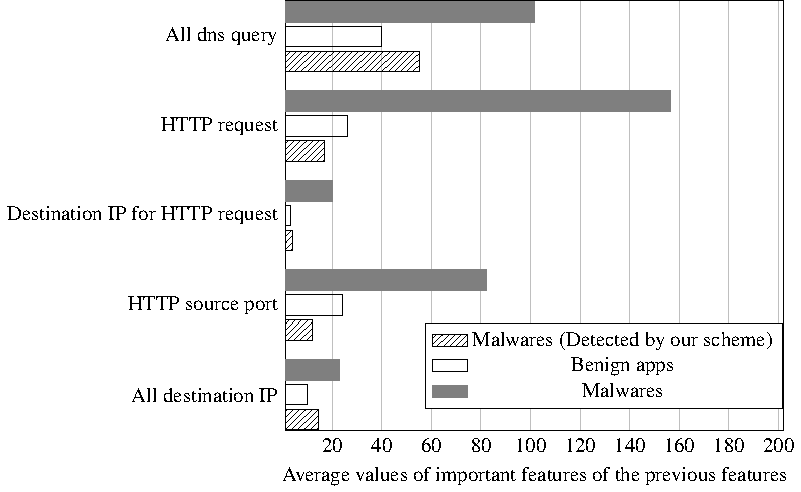
\includegraphics[scale=1.0, bb=10 10 250 250]{./figures/important_prev_f_tikz.pdf}
  \caption{Average values of top 5 important previous features} 
  \label{fig:important_prev_feature}
\end{figure}

As shown in \figurename~\ref{fig:important_prev_feature}, these features of the malwares detected by \our scheme are similar to the benign ones.
% Thus, the previous scheme cannot detect such malwares.
% Meanwhile, Prop.1 can deal with the malwares whose traffic patterns are similar to benign ones because strong evidence of malwares can be extracted from the destination server. 
\Our scheme can detect such malwares including repackaged malwares because strong evidence of malwares can be obtained from \our features based on the relation between dangerous permissions and the level of SSL server certificates. 
Furthermore, \we manually check SSL server certificate and traffic data of the malwares detected only by \our scheme.
After that, \we discovered the malwares that communicate with an unknown server and send device information to the server.
This result means that \our scheme is applicable to encrypted data because the malwares which send sensitive information can be detected without packet inspection.
Accordingly, \we conclude that \our scheme can deal with the shortcoming of the previous scheme and encrypted data.
Furthermore, \we evaluate the scheme combining \our scheme and the previous scheme.
As show in \tablename~\ref{tab:result}, the scheme achieves best detection performance in our evaluation.
Hence, \we conclude that \our scheme and the previous scheme are complementary, and a hybrid scheme can more improve detection performance.
% Since the level of SSL server certificates introduced to the servers of attackers is hard to be disguised by them, malwares cannot easily evade indicating malicious evidence.
% Thus, even if attackers disguise traffic patterns of malwares, Prop.1 can detect the malwares.  
\afterpage{\clearpage}
\newpage
\section{Evaluation of permission base weight values} 
In order to demonstrate whether permission based weight values are effective, \we evaluate the detection performance of SSL certificate based scheme and the permission based scheme.
As shown in \tablename~\ref{tab:result}, in comparison to \our scheme, SSL certificate based scheme degrades detection performance regarding accuracy, TPR and FPR.
Because the benign apps may communicate with DV and unknown servers, SSL certificate based scheme misjudges such benign apps as malwares.
\Our scheme can correctly judge such benign apps by considering required permissions because they do not require dangerous permissions.
Meanwhile, although the permission based scheme can correctly judge benign apps with low FPR, TPR is degraded in comparison to the other schemes.
This is because that scheme is not applicable to repackaged malwares.
After manually checking the dangerous permissions required by the repackaged malwares and original apps, \we confirm that most repackaged malwares have the permissions required by original apps.
\Our scheme can detect such repackaged malwares because \our features indicate strong evidence of malwares by combining SSL server certificate based features and required dangerous permissions.
% Thus, Prop.1 can correctly judge such benign apps due to permission based weight values.  
Thus, \we conclude that assigning permission based weight values to SSL server certificate based features is effective in improving detection performance.  
\afterpage{\clearpage}
\newpage

\section{False Positive Analysis}
\Our scheme regards 73 benign apps as malwares in \our simulation (i.e., false positives).
After manually analyzing these false positives, \we discovered that the app sending sensitive information such as IMEI which is the unique identifier of the phone to a unknown server while the app is labeled as benign one by VirusTotal.
\we conclude that the app is a malware since the app sends sensitive information to untrusted servers. 
\We send the app to VirusTotal again in order to confirm the newest detection result of VirusTotal for the app because the detection results of VirusTotal have been updated continuously.
Accordingly, 60 antivirus scanners in VirusTotal do not rise any alarm for the app.
Therefore, the app is still regarded as benign one by VirusTotal.
Furthermore, the previous scheme also labels the app as benign one.
From these result, \we conclude that \our scheme can detect the malwares which evade 60 antivirus scanner and the previous scheme by using \our features.  

\afterpage{\clearpage}
\newpage

\section{False Negative Analysis} 
\Our scheme misses 106 malwares, while 36 of them can be detected by the previous scheme.
After manually checking the level of SSL server certificate and traffic data, \we discovered that these malwares do not interact with untrusted servers.
This is because \we cannot bring out malicious actions of malwares.
Some malwares do not conduct malicious actions on an emulator to escape detection.
Thus, these inspection results reveal the limitation of \our scheme. 
% Thus, in order to inspect these malwares, \we need to excute them on a real device in the future.

